%!TeX root=../tese.tex
%("dica" para o editor de texto: este arquivo é parte de um documento maior)
% para saber mais: https://tex.stackexchange.com/q/78101

%% ------------------------------------------------------------------------- %%

\chapter{Conclusão}
\label{cap:conclusao}

Aprendizado de máquina, e principalmente aprendizado por reforço, nem sempre é capaz de chegar ao resultado esperado e infelizmente este trabalho é um desses casos. Isso acontece por diversos motivos, mas os principais são uma alta complexidade a qual faz com que o aprendizado precise de muito tempo para convergir e o sistema, mais comumente em aprendizagem por reforço, pode aprender um comportamento diferente do desejado. Este trabalho simplifica o aprendizado ao reduzir o número de ações possíveis, porém não é capaz de gerar regras para recompensar o robô de forma que incentive o modelo a aprender a percorrer o circuito ao invés de ficar girando em círculos ou valer-se de outra forma para maximizar a pontuação.

\begin{figure}
	\centering
	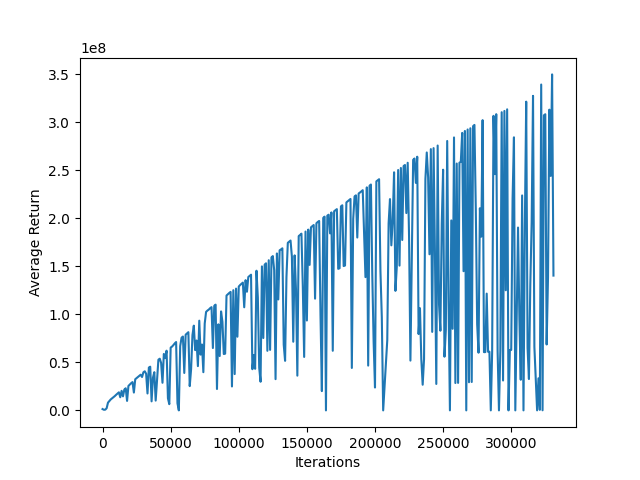
\includegraphics[width=.8\textwidth]{grafico_pontuacao}
	\caption{Gráfico da evolução durante sessão de treino. \label{fig:grafico_pontuacao}}
\end{figure}

Outro grande problema é a grande instabilidade do modelo durante as sessões de treinamento, como pode ser observado na figura ~\ref{fig:grafico_pontuacao}. Tal instabilidade na pontuação não parece ser proveniente da alta bonificação dada quando o robô avança para uma nova casa da pista mas das formas que ele encontra para tirar proveito do sistema de pontuação, o que por sua vez dificulta analisar a evolução ou regressão do robô. Finalmente, mesmo com as simplificações e mudanças do modelo o processo de aprendizagem ainda leva muito tempo para gerar resultados conclusivos sobre o desempenho do robô, assim faz com que seja necessário um gasto muito grande de tempo para poder determinar se o comportamento visto é originário de uma má pontuação ou do comportamento aleatório aprendido enquanto se explora o ambiente.

Em síntese, para obter resultados mais satisfatórios se faz necessário um maior desenvolvimento do projeto a fim de remover as insuficiências do modelo. Dessa maneira, é fundamental a implementação de novos métodos de otimização que sejam capazes de acelerar o processo de aprendizado de forma que se torne possível uma mais rápida avaliação da evolução do treinamento da rede neural e, por conseguinte, a reavaliação dos critérios de pontuação. Por último, também é de suma importância um estudo mais aprofundado em tecnicas para fazer um melhor sistema de pontuação para aprendizado, em virtude de estabelecer melhores parâmetros de avaliação da evolução da rede além de permitir a localização com uma maior exatidão da causa do comportamento inesperado aprendido pelo robô.
